% TCM: TOTEM Communication Middleware
% Copyright: Copyright (C) 2009-2012
% Contact: denis.conan@telecom-sudparis.eu, michel.simatic@telecom-sudparis.eu
% Permission is granted to copy, distribute and/or modify this document
% under the terms of the GNU Free Documentation License, Version 1.3
% or any later version published by the Free Software Foundation;
% with no Invariant Sections, no Front-Cover Texts, and no Back-Cover Texts.
% A copy of the license is included in the section entitled "GNU
% Free Documentation License".


\section{Example application demonstrating the integration of the technologies}
\label{S_integration}

This section presents an illustrative application that demonstrates
the communication technologies of the TOTEM project. The section
focuses on technologies, design patterns and idioms, not on
``business'' functionalities for game applications.

\subsection{Analysis}
\label{SS_integration_analysis}

\subsubsection{Subsystems, use cases and scenarios}
\label{SSS_integration_subsystems}

Figure~\ref{F_use_case} of Section~\ref{S_use_case} presents the use
cases of the illustrative application.
Figure~\ref{F_integration_use_case_game_server} lists the
functionalities of the \textsf{Game Server} and \textsf{Logging
  Server}. For the sake of simplicity, the use cases of the
\textsf{Master Application}, the \textsf{Player Application} and
\textsf{Spectator Application} are the ones accessed by these
subsystems in Figure~\ref{F_integration_use_case_game_server}.

\begin{figure}[htbp!]
\begin{center}
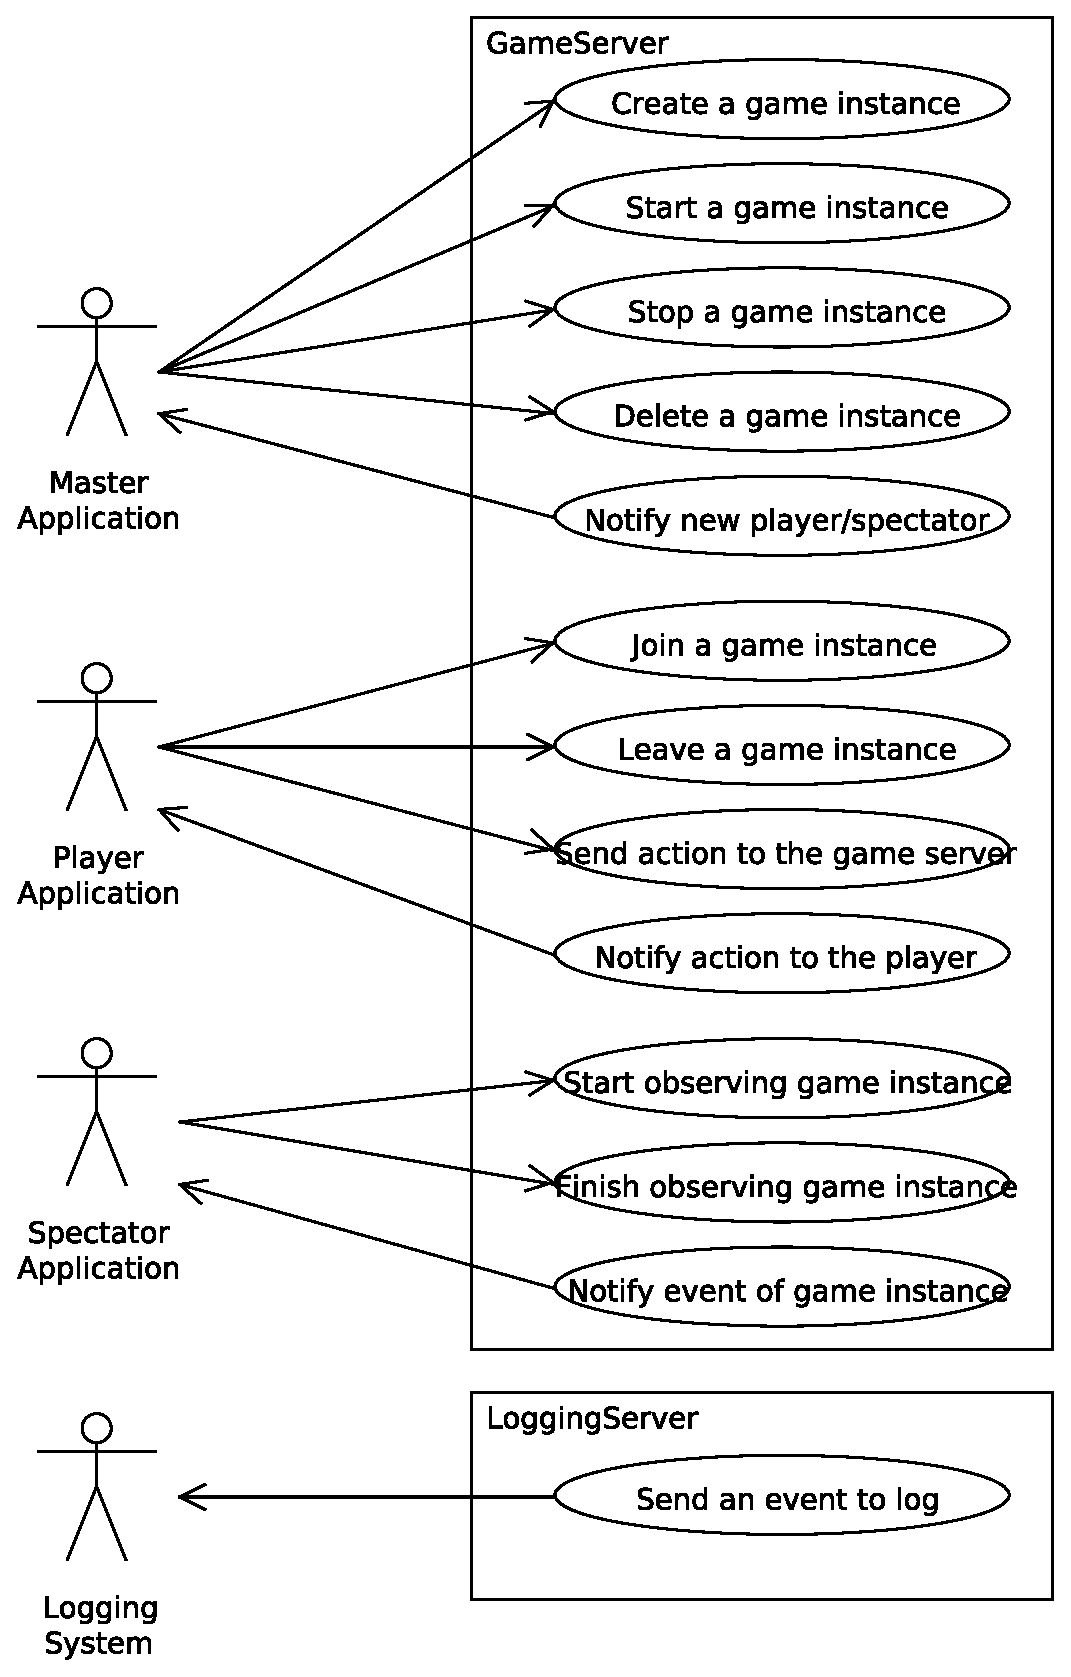
\includegraphics[scale=0.55]{Figures/_integration_use_case_game_server}
\caption{Use case diagram of the subsystem \textsf{Game Server}}
\label{F_integration_use_case_game_server}
\end{center}
\end{figure}

\newpage

The scenarios are modelled into activity diagrams:
\begin{itemize}
\item Figure~\ref{F_integration_activity_create_join} depicts the
  steps of the creation of the game and the game instances, and then
  the steps up to the beginning of the game, that is the period
  during which players and spectators can join the game instance. The
  signals are colored according to the emitter or the receiver:
  magenta is for game masters, cyan is for spectators and yellow is
  for players. Note that the game master that creates a game and the
  game master that creates a game instance may be two different
  participants; in Figure~\ref{F_integration_activity_create_join}, they
  are named $m_1$ and $m_2$, respectively.
\item Figure~\ref{F_integration_activity_be_informed_new_game_instance}
  explains how a player is informed about the list of game instances
  that she can join, and how she ask for joining the chosen game
  instance as player. A similar activity diagram can be drawn to model
  how a spectator chooses the game instance and how she ask for
  joining as a spectator.
\item Figure~\ref{F_integration_activity_leave_game_instance} shows the
  end of a game instance when the game master asks for its closure.
\end{itemize}

\begin{figure}[htbp!]
\begin{center}
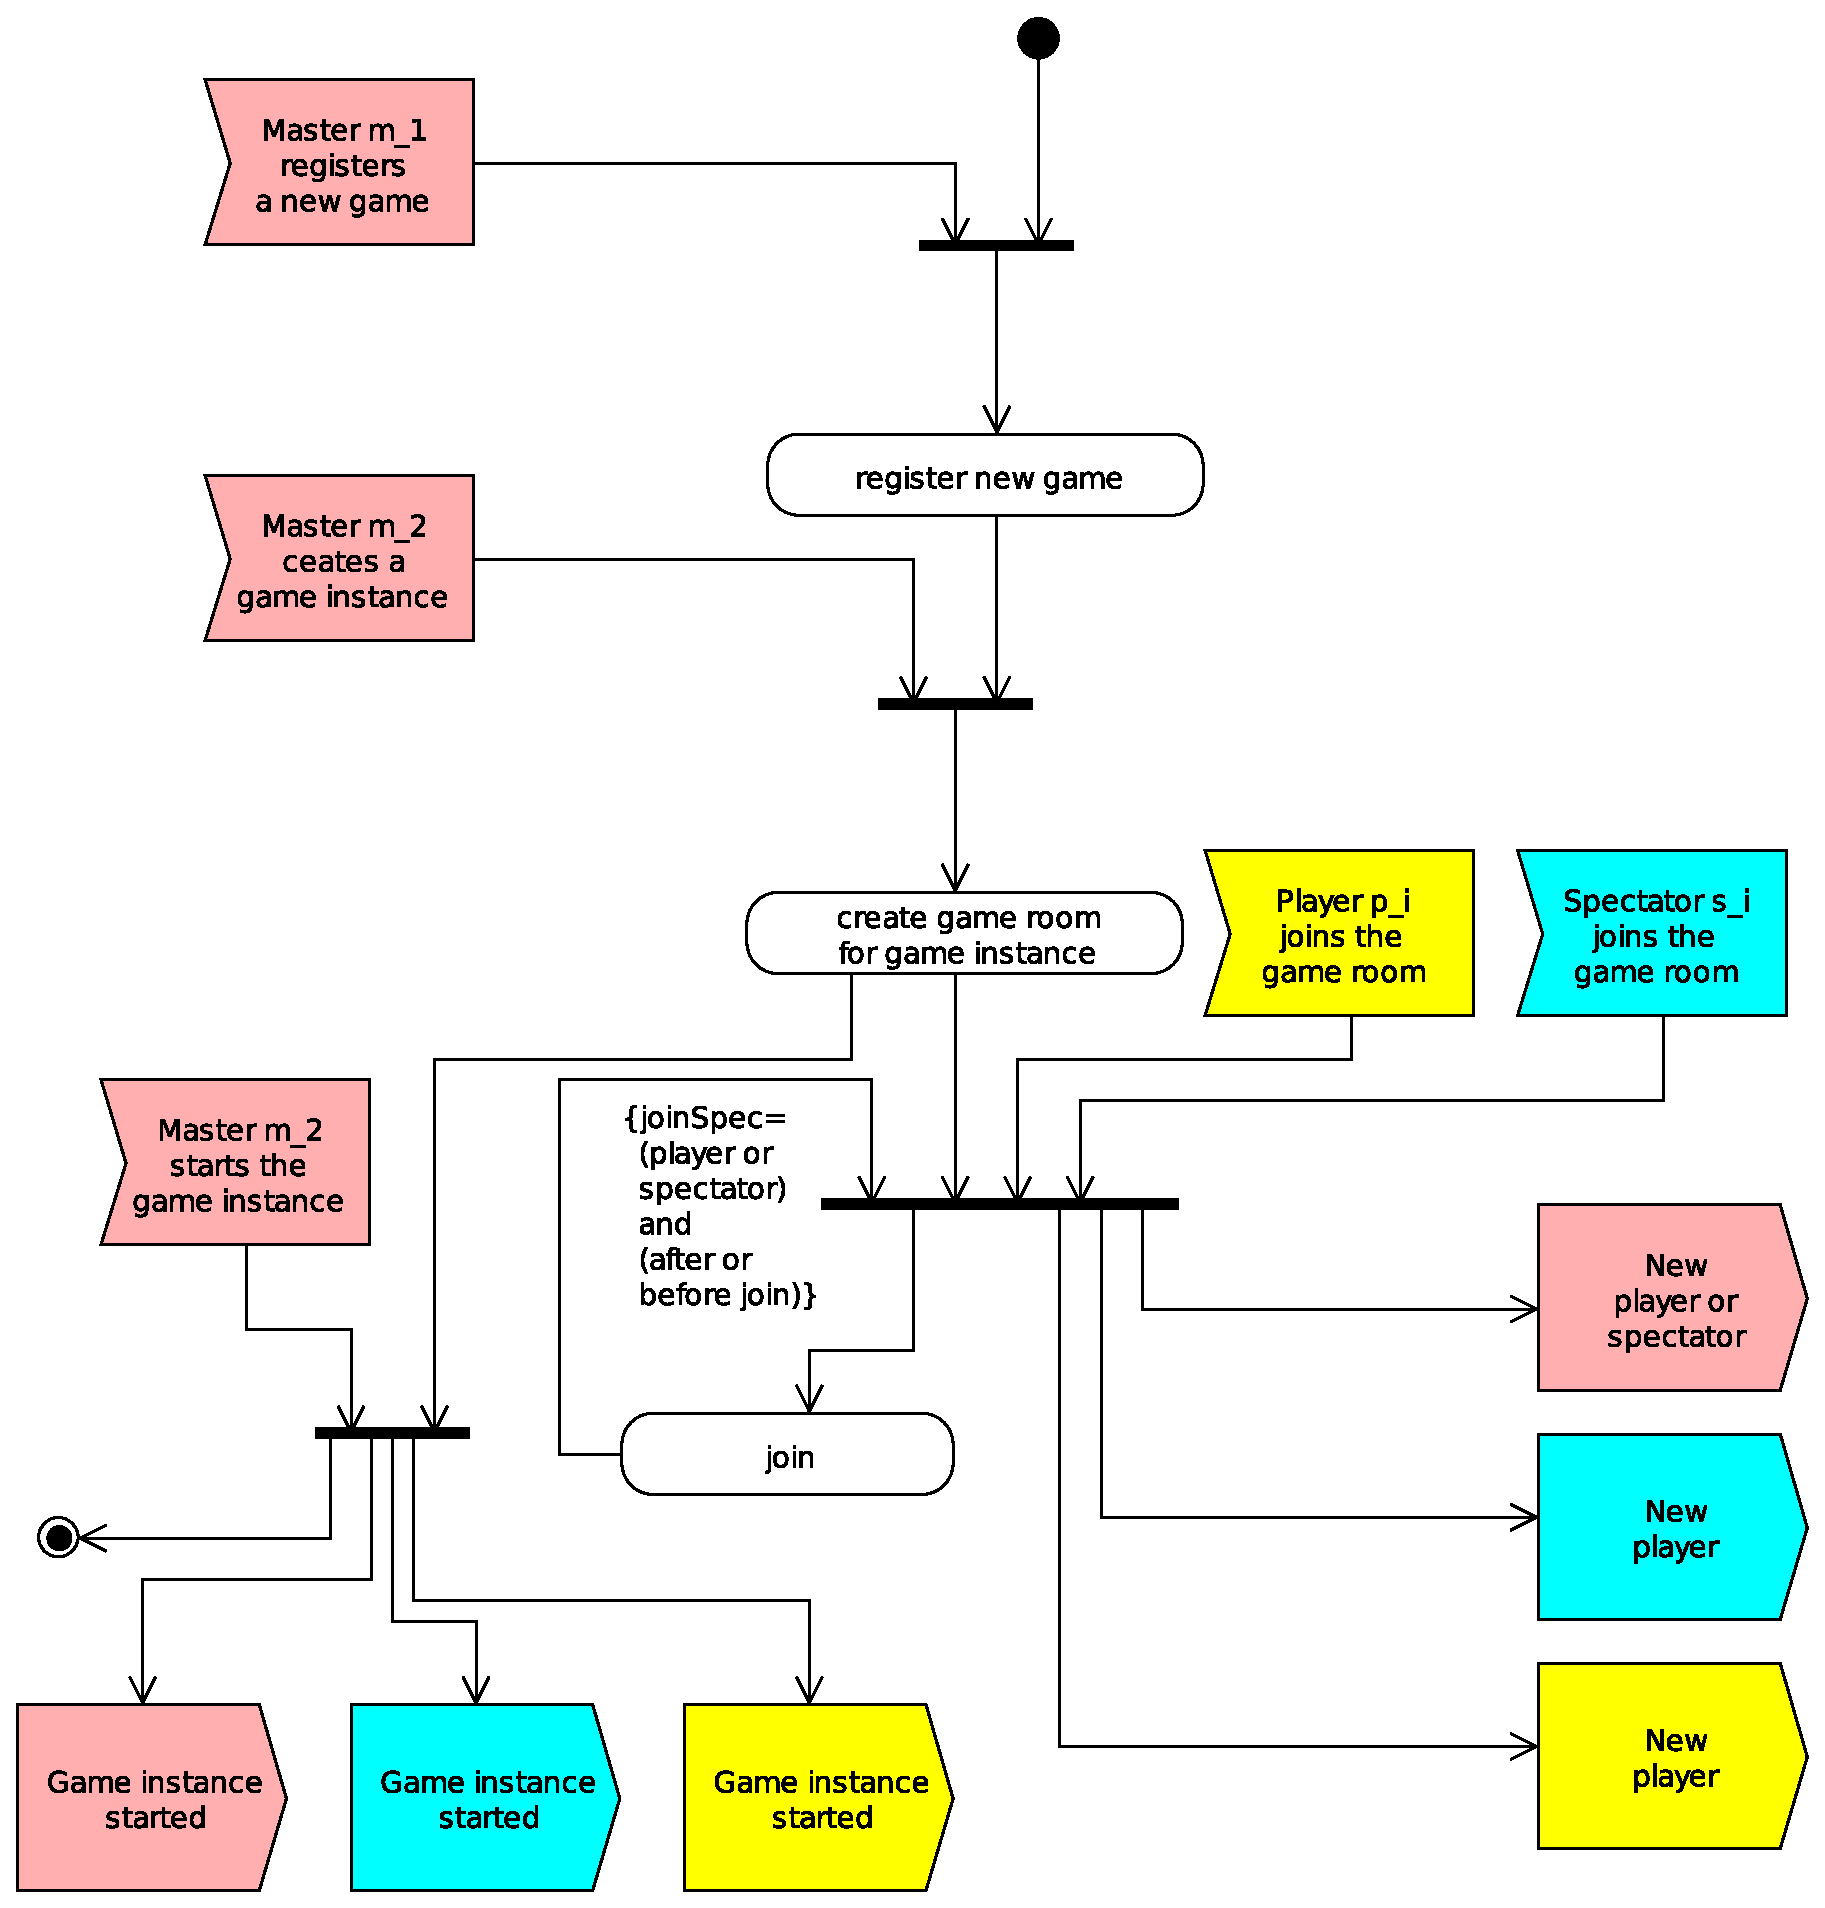
\includegraphics[scale=0.5]{Figures/_integration_activity_create_join_game_instance}
\caption{Activity diagram of the creation of the game and the game
  instance, and of the joining of players and spectators}
\label{F_integration_activity_create_join}
\end{center}
\end{figure}

\begin{figure}[htbp!]
\begin{center}
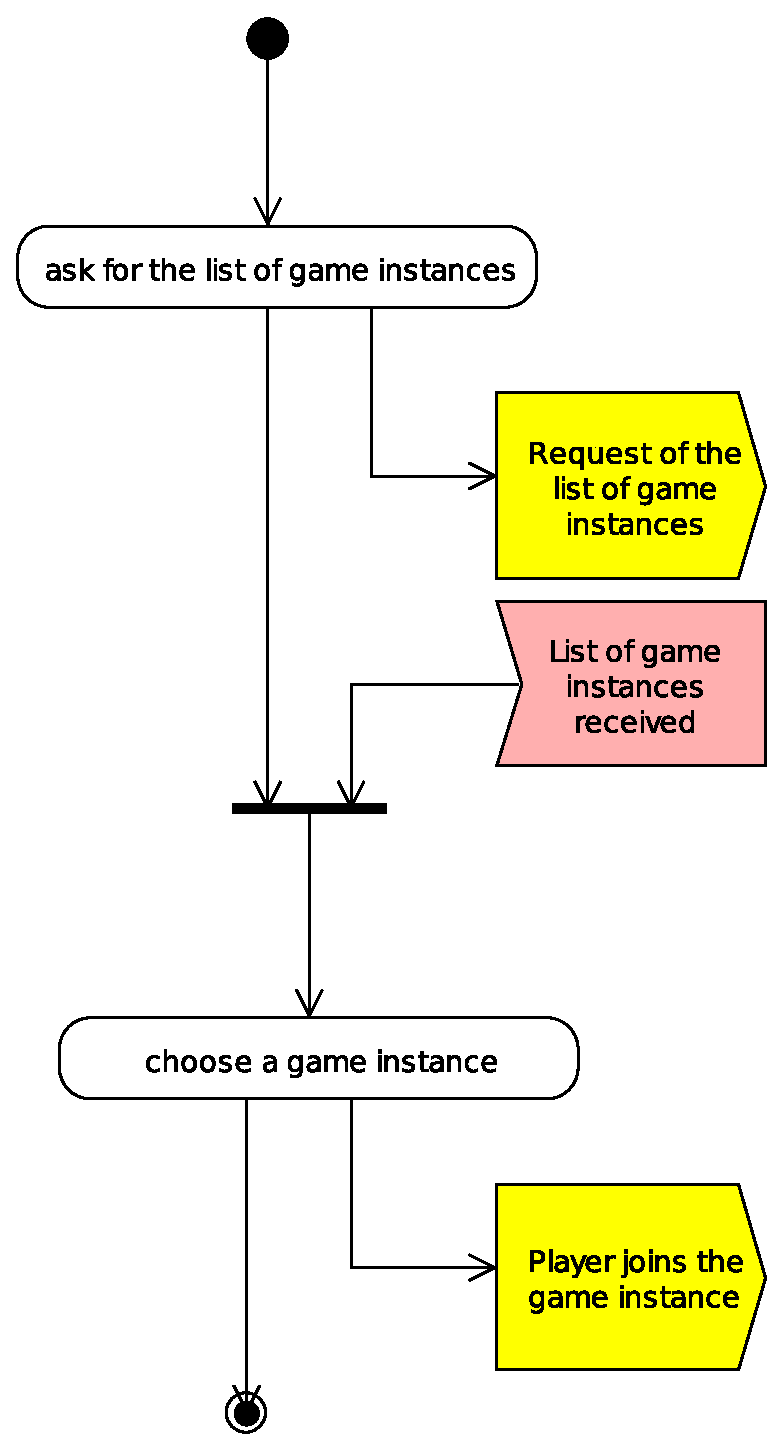
\includegraphics[scale=0.5]{Figures/_integration_activity_be_informed_new_game_instance}
\caption{Activity diagram of how a player is informed about and
  chooses a game instance}
\label{F_integration_activity_be_informed_new_game_instance}
\end{center}
\end{figure}

\begin{figure}[htbp!]
\begin{center}
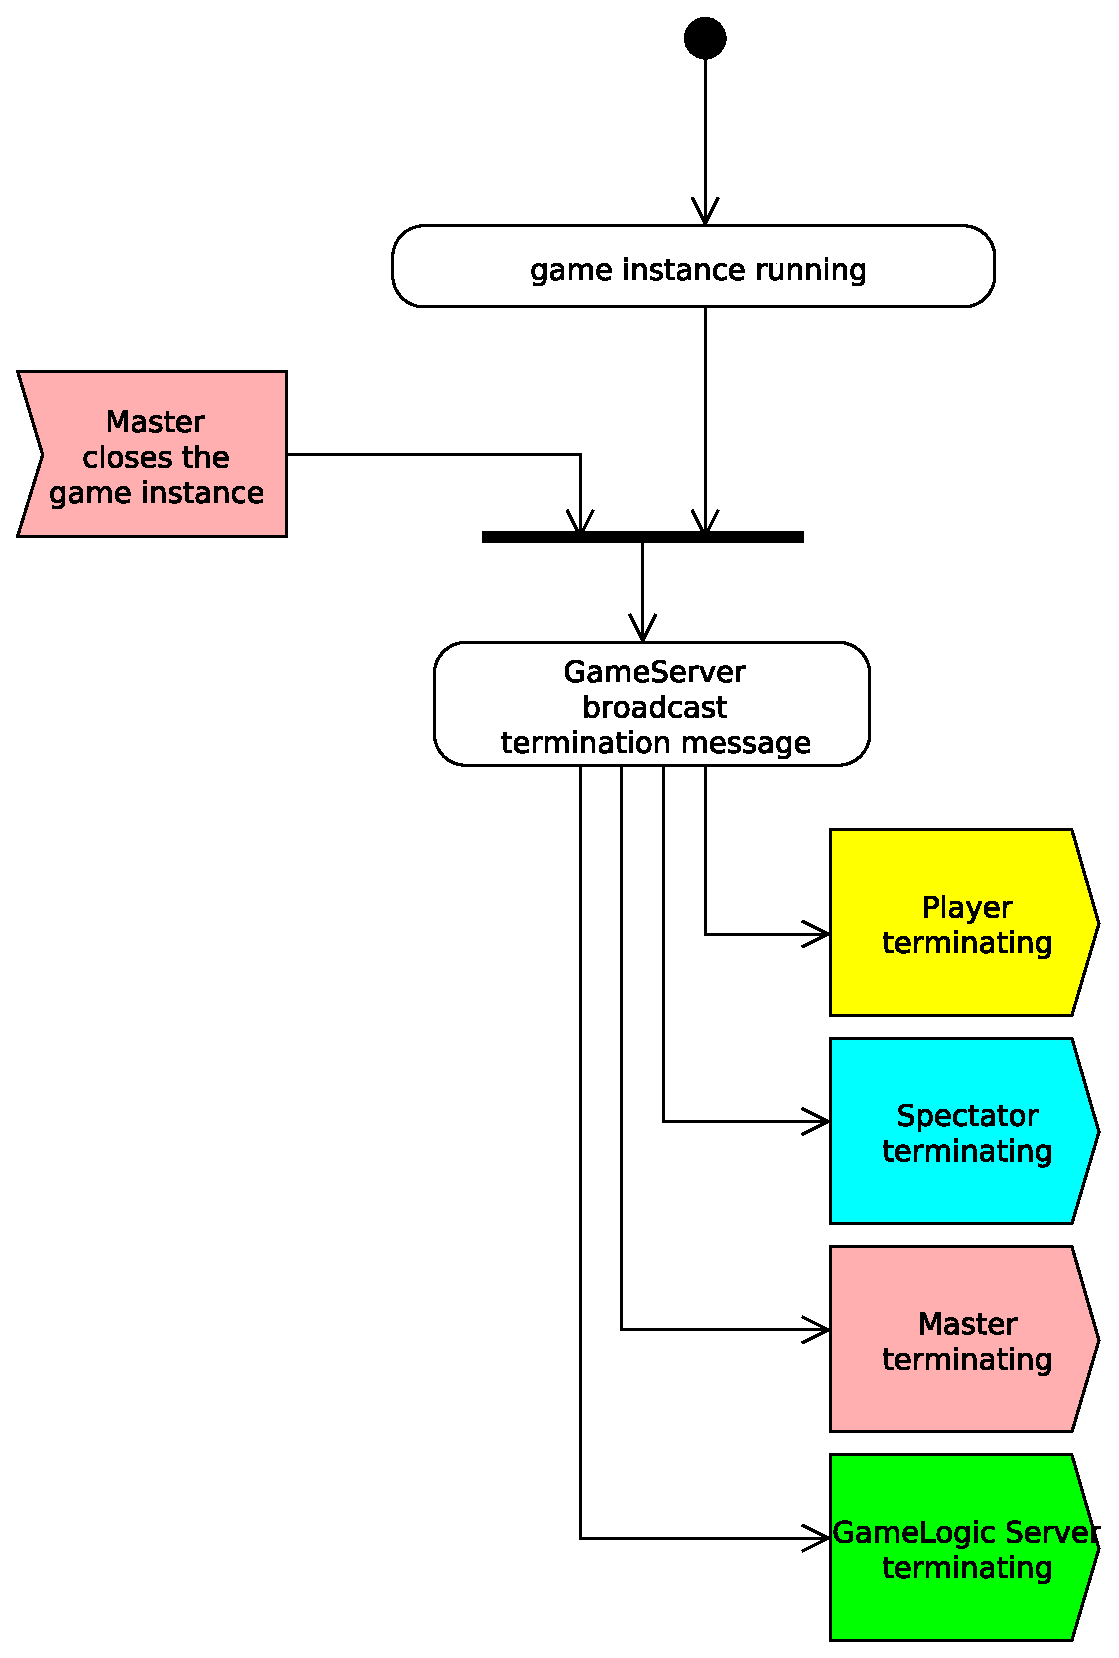
\includegraphics[scale=0.5]{Figures/_integration_activity_leave_game_instance}
\caption{Activity diagram of the end of the game instance}
\label{F_integration_activity_leave_game_instance}
\end{center}
\end{figure}

\newpage

\subsubsection{Business classes}
\label{SSS_integration_analysis}

The static aspects of the analysis of the system is presented in the
class diagram of Figure~\ref{F_integration_class}. This model is very
simple since we have simplified the business concerns in order to
focus on the architectural aspects of the communication part. A \textsf{Game} is
specified by providing a \textsf{name} only. It can be ``played''
several times (possibly in parallel), leading to several
\textsf{Game Instance}s. Each \textsf{Game Instance} is created and
controlled by a \textsf{Participant} called the \textsf{master},
involves several \textsf{Participant}s that are the \textsf{player}s,
and can be followed by other \textsf{Participant}s called the
\textsf{spectator}s. A \textsf{Participant} can take part to several
\textsf{Game Instances} either as \textsf{master}, \textsf{player} or
\textsf{spectator}. A logged message, named a \textsf{Log} for short,
is related to a \textsf{Game Instance} and a \textsf{Participant}. Not
explicitly shown in this diagram, we will allow the logging of purely
``technical messages'' from all the subsystems and that do not concern
a particular \textsf{Game Instance} or a specific
\textsf{Participant}; this is why the multiplicity of the associations
connected to the class \textsf{Log} are ``$0..n$''.

NB~1: In this illustrative application demonstrating the integration of
the different technologies into a consistant communication
architecture, we ignore rights management. In other words, every
participant can be a master and every participant can be a player or a
spectator of every game instance. The \textsf{login} and
\textsf{password} attributes of the class \textsf{Participant} serves
to have access to the communication infrastructure.

NB~2: In this illustrative application, for the sake of simplicity, we
log only events/messages that belong to a game instance.

NB~3: In this illustrative application, no information is stored in a
database, thus there is no database access. This should not be the case
if the application is integrated into the TOTEM \textsf{Django} game
server.

\begin{figure}[htbp!]
\begin{center}
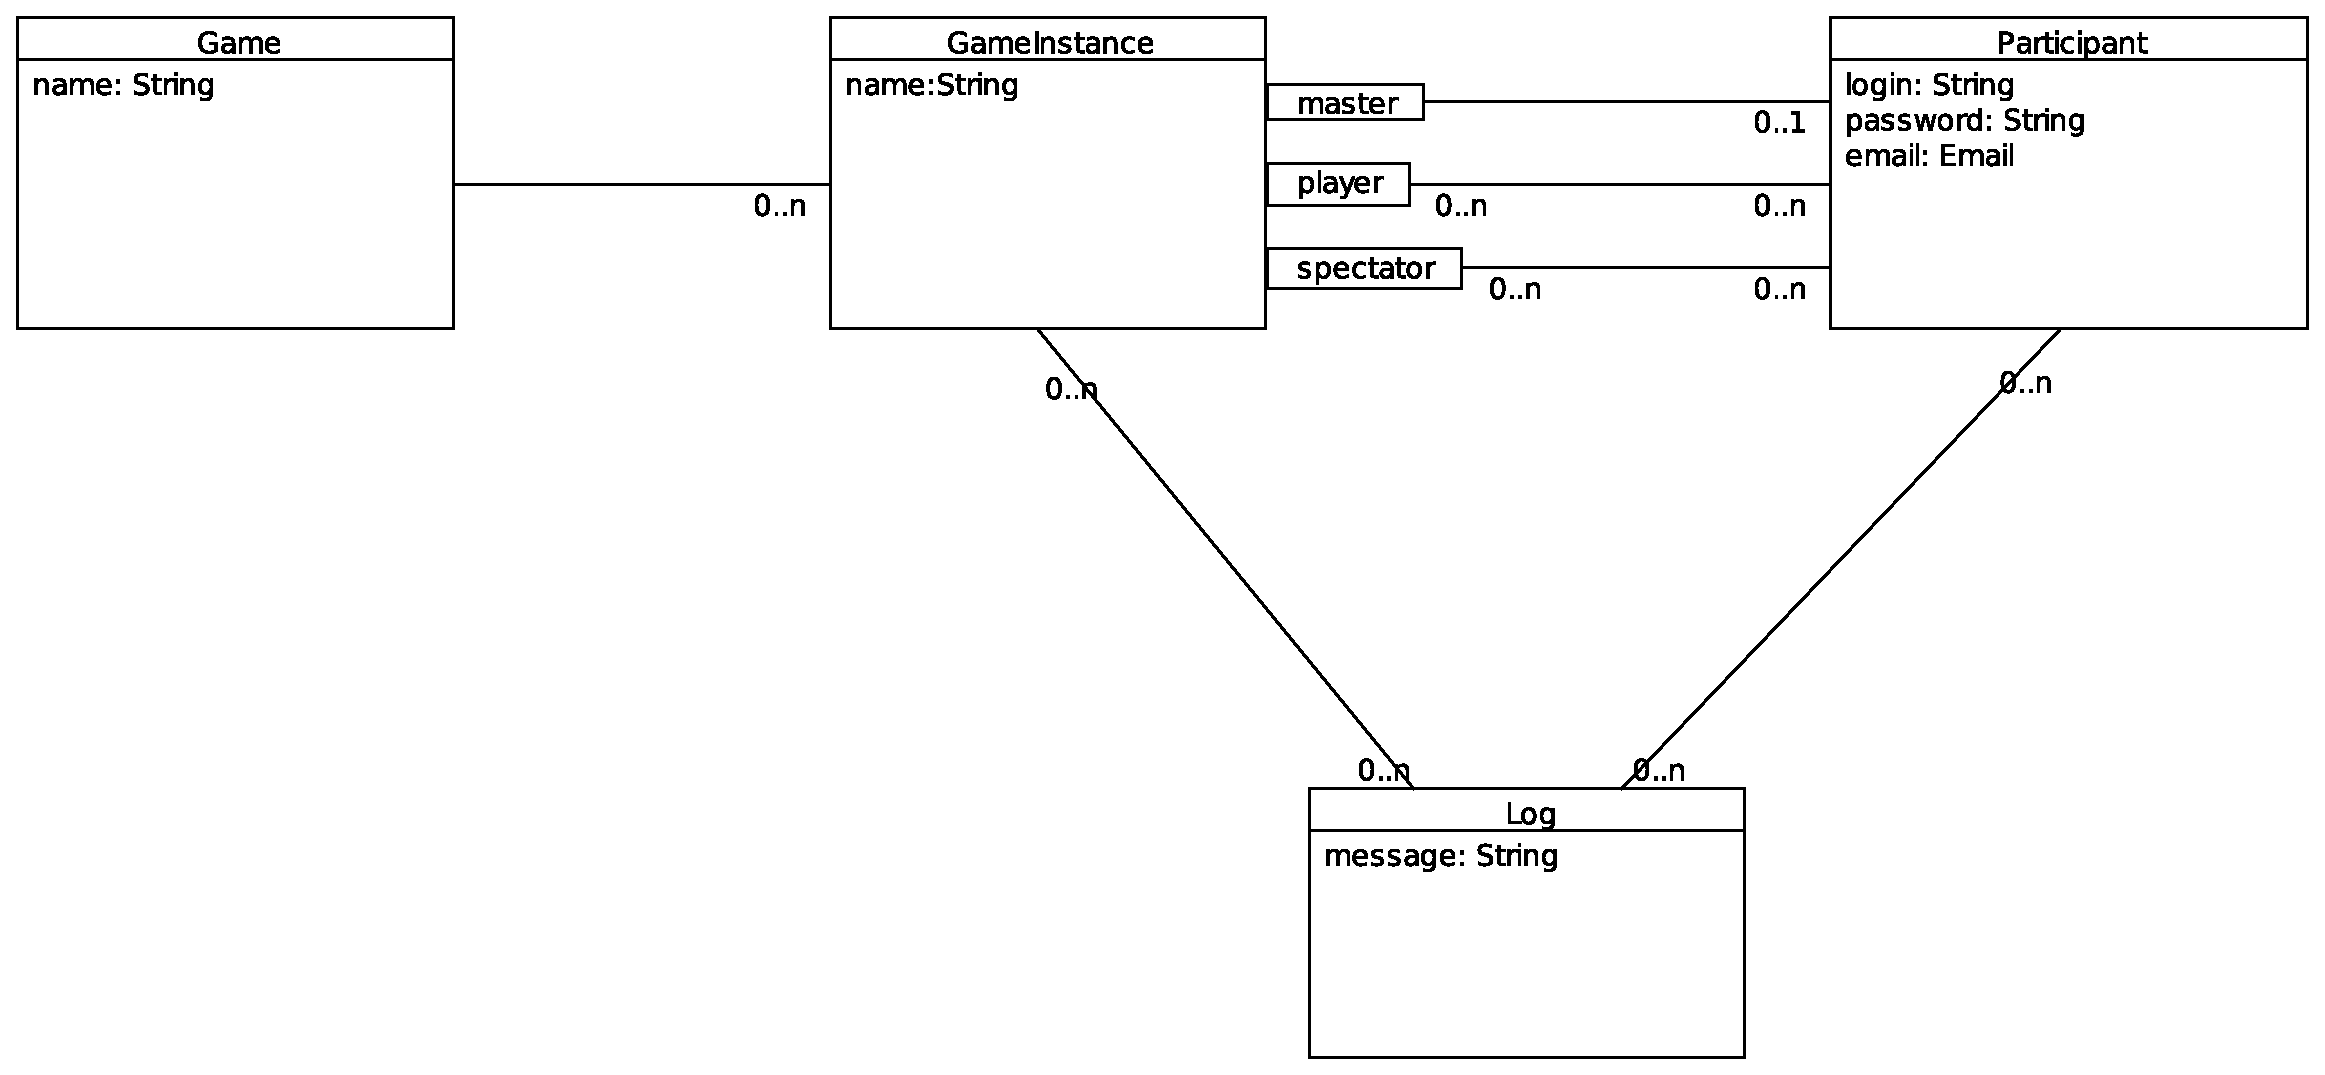
\includegraphics[scale=0.4]{Figures/_integration_class}
\caption{Class diagram of the business concepts used in the subsystems}
\label{F_integration_class}
\end{center}
\end{figure}

\newpage

\subsection{Design of the communication architecture for the game instance}
\label{SS_integration_design}

During a game instance, messages are exchanged through the event-based
system whose configuration is presented in
Figure~\ref{F_architecture_game_instance} (a game instance with a game
logic server, one game master, two players, two spectators, and the
logging mechanism activated). The figure uses the following concepts
from AMQP:
\begin{itemize}
\item The identifier of the game instance serves as the name of the
  virtual host. There is one virtual host per game instance so that
  game executions do not interfer.
\item The first entity in the system is the \textsf{Game Logic
  Server}. It is responsible for creating the topic exchange and the
  queues.
\item Every participant (game master, players, spectators, and logging
  services) has a dedicated queue to receive events.
\item The topic exchange allows filtering with routing keys decomposed
  into four parts: the identifier of the sender (for instance,
  \textsf{p1}), the identifier of the receiver (for instance,
  \textsf{m1}), the kind of action transported in the
  event (for instance, \textsf{join}), and the name of the
  action (for instance, \textsf{joinMaster}).
\item The \textsf{Game Logic Server}, the game master, and the players
  have two bindings: for instance \texttt{*.m1.\#} for receiving
  messages sent only to them, and \texttt{*.all.\#} for receiving
  broadcast messages.
\end{itemize}

The creation and the management of the game instance communication
architecture is described in the following figures:
\begin{itemize}
\item Figure~\ref{F_integration_sequence_game_instance_1} presents the
  sequence diagram of the creation of the game instance and of the
  joining of the \textsf{Master Application} to the game
  instance. The \textsf{Master Application} sends an XMLRPC request to
  the \textsf{Game Server}. The \textsf{Game Server} creates the
  \textsf{Game Logic Server} process. This process is responsible for
  creating the AMQP communication infrastructure and creating the
  thread \textsf{XMLRPC Worker}, which is reponsible for performing
  the join action of the actors. The \textsf{Game Server} and the
  \textsf{Game Logic Server} synchronize using a semaphore so that the
  first join operations are not called before the virtual host and the
  exchange are created.  Figure~\ref{F_architecture_game_instance_1}
  displays the architecture after the creation of the game instance.
  Next, Figure~\ref{F_architecture_game_instance_2} depicts the new
  architecture of the application instance when the \textsf{Master
    Application} has joined the application instance.
\item Figure~\ref{F_integration_sequence_game_instance_2} presents the
  sequence diagram of the joining of a \textsf{Spectator Application}
  to the game instance. The \textsf{Spectator Application} sends an
  XML-RPC request to the \textsf{Game Server} that forwards it to the
  \textsf{XMLRPC Worker} thread of the \textsf{Game Logic
    Server}. Figure~\ref{F_architecture_game_instance_3} depicts the
  new architecture of the application instance when the
  \textsf{Spectator Application} has joined the application instance.
\item Figure~\ref{F_integration_sequence_game_instance_3} presents the
  sequence diagram of the joining a \textsf{Player Application} to the
  game. The \textsf{Player Application} sends an XMLRPC request to the
  \textsf{Game Server} that forwards it to the \textsf{XMLRPC Worker}
  thread of the \textsf{Game Logic
    Server}. Figure~\ref{F_architecture_game_instance_4} depicts the
  new architecture of the application instance when the
  \textsf{Player Application} has joined the application
  instance.
\end{itemize}

NB: in all the models of this section, for the sake of simplicity, we
assume that the actors know their identity and obtain the information
about games and game instances from another means, for instance from
the Web framework. We also assume that they have unique identities
and that their login names do not contain any dot (since the login
names are used for binding and routing keys).

\begin{figure}[htbp!]
\begin{center}
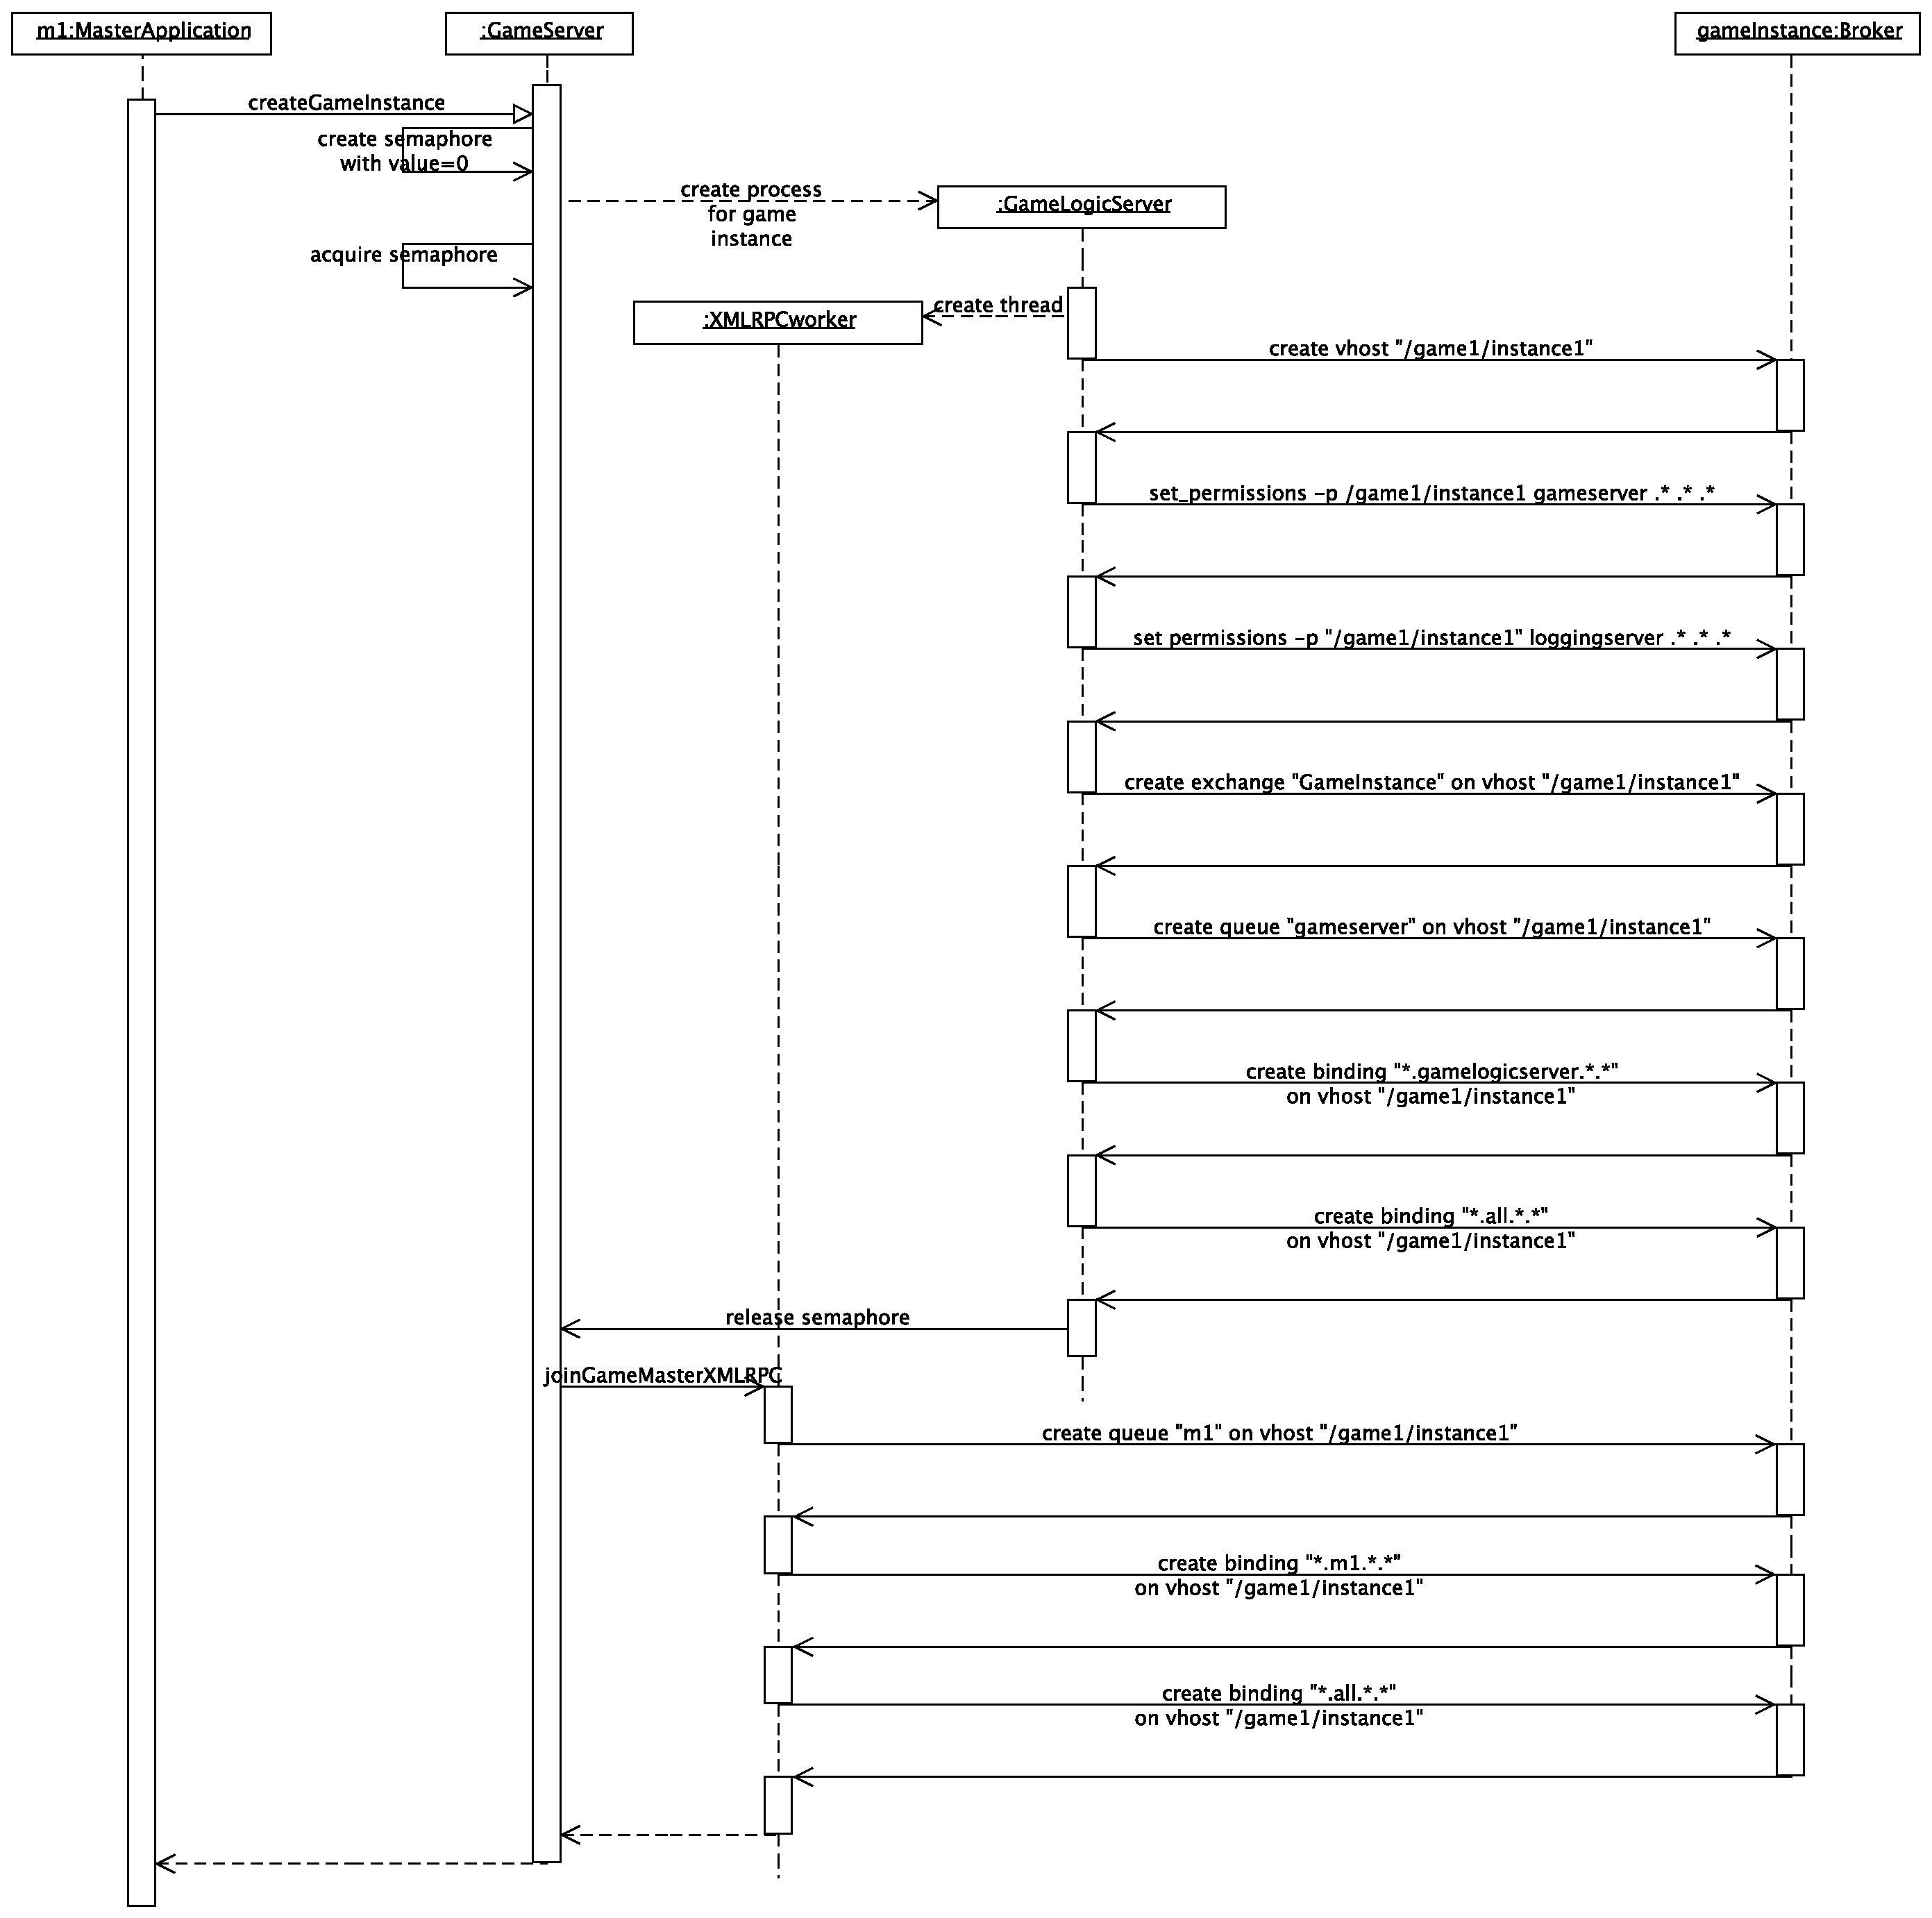
\includegraphics[scale=0.4]{Figures/_integration_sequence_game_instance_1}
\caption{Sequence diagram of the creation of the game instance}
\label{F_integration_sequence_game_instance_1}
\end{center}
\end{figure}

\begin{figure}[htbp!]
\begin{center}
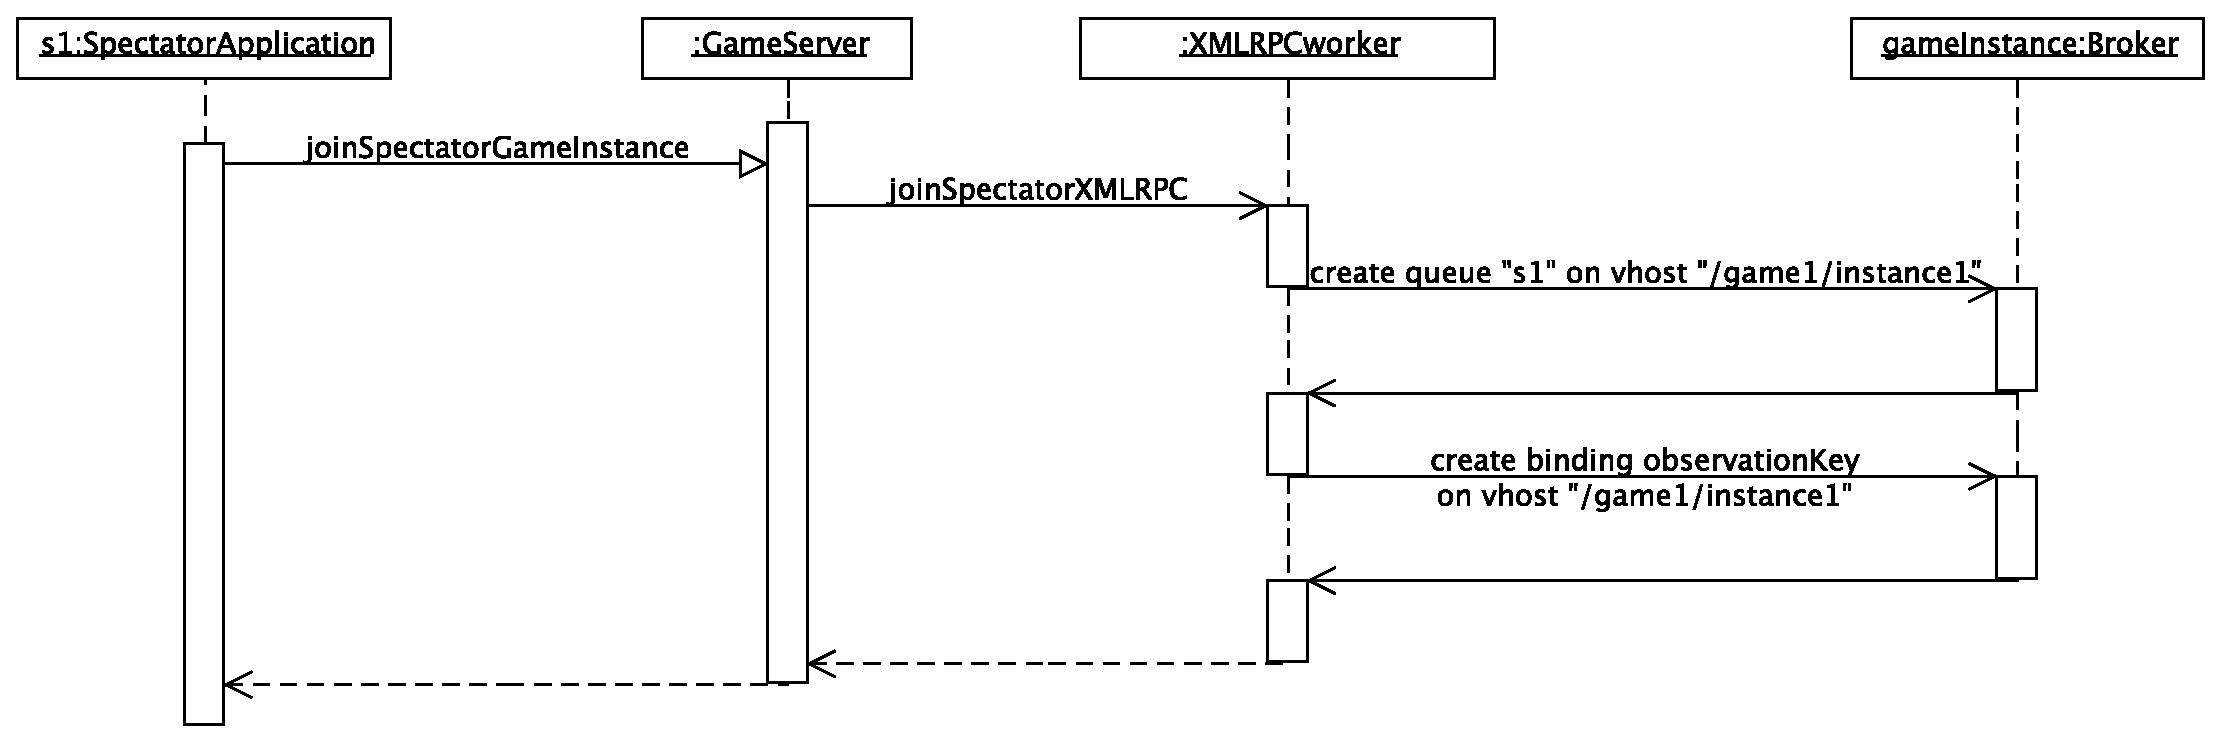
\includegraphics[scale=0.4]{Figures/_integration_sequence_game_instance_2}
\caption{Sequence diagram of the joining of the \textsf{Spectator
    Application} to the game instance}
\label{F_integration_sequence_game_instance_2}
\end{center}
\end{figure}

\begin{figure}[htbp!]
\begin{center}
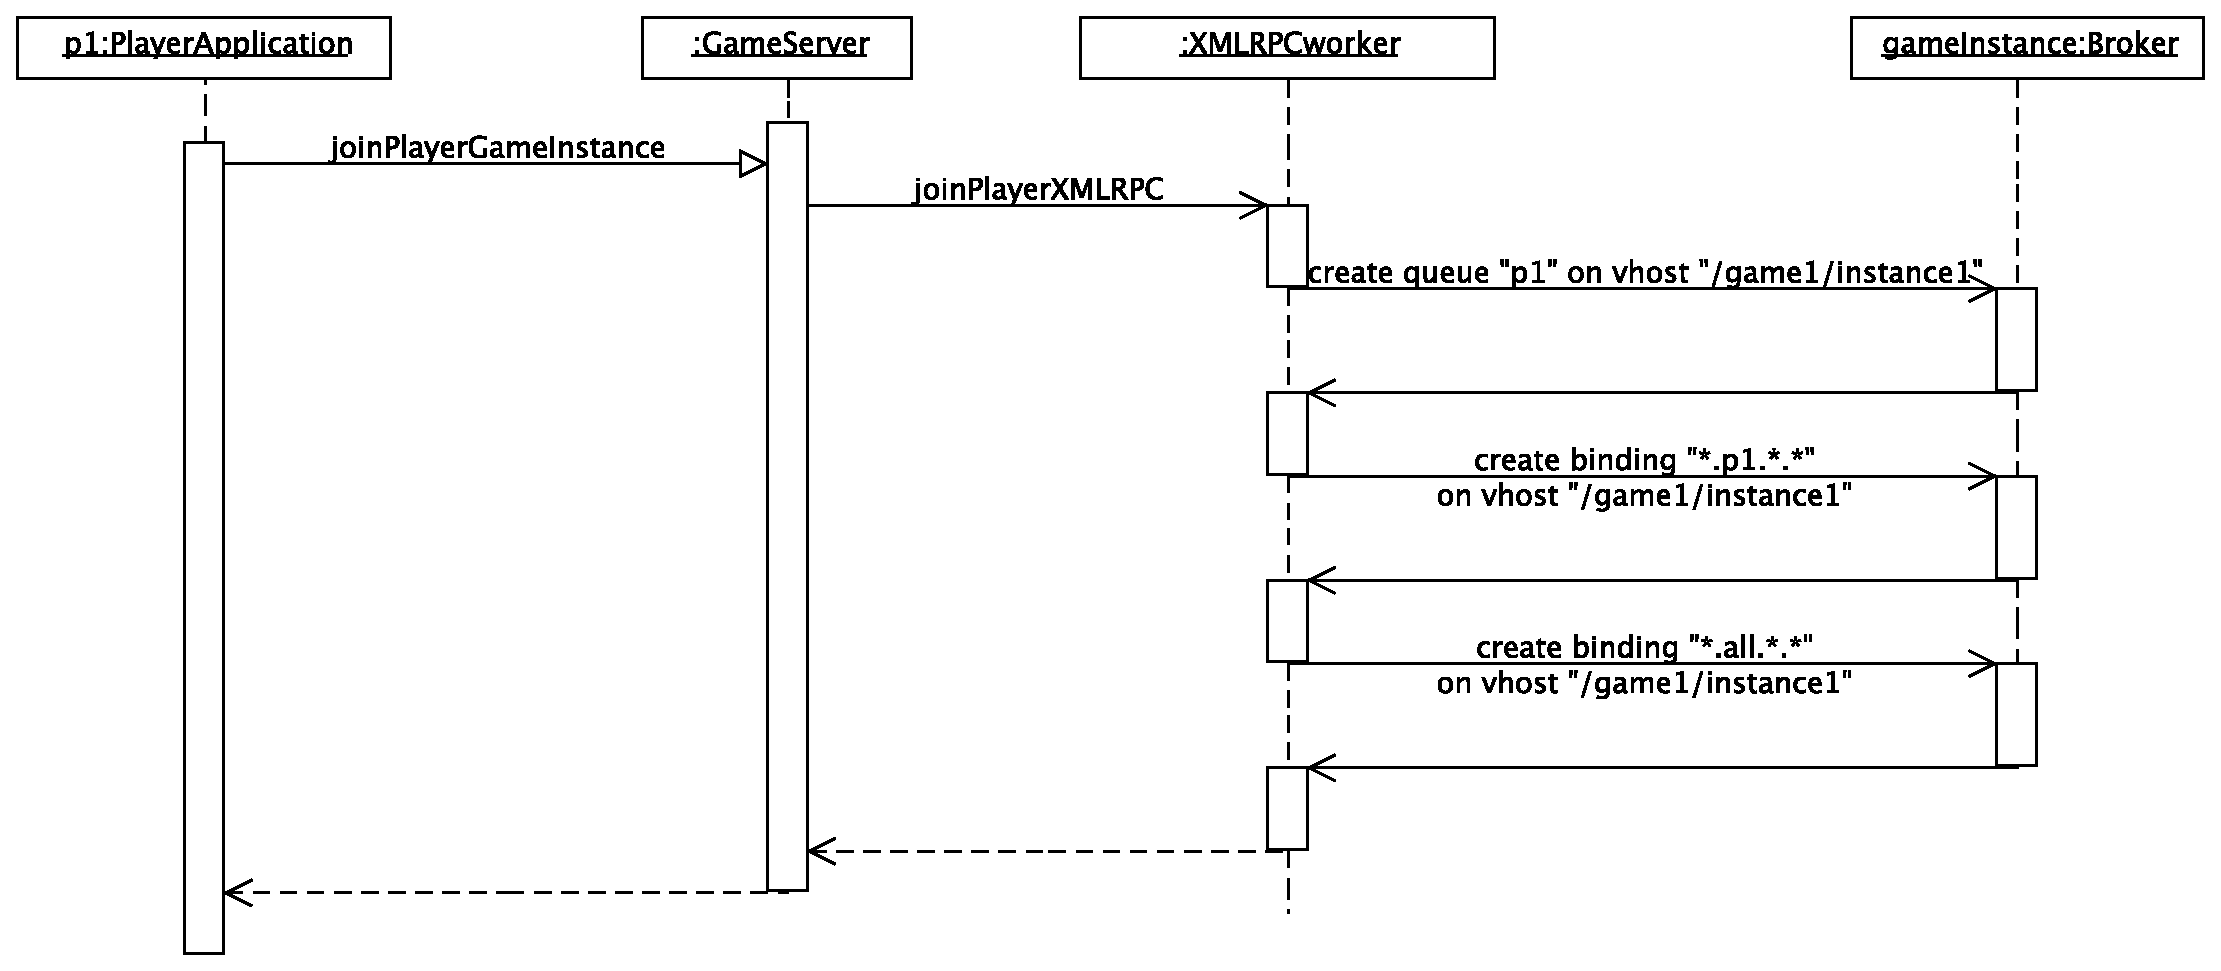
\includegraphics[scale=0.4]{Figures/_integration_sequence_game_instance_3}
\caption{Sequence diagram of the joining of a \textsf{Player
    Application} to the game instance}
\label{F_integration_sequence_game_instance_3}
\end{center}
\end{figure}

\begin{figure}[htbp!]
\begin{center}
\includegraphics[scale=0.6,angle=90]{Figures/architecture_game_instance_1}
\caption{Architecture of the subsystem for the game instance
  (at creation time)}
\label{F_architecture_game_instance_1}
\end{center}
\end{figure}

\begin{figure}[htbp!]
\begin{center}
\includegraphics[scale=0.6,angle=90]{Figures/architecture_game_instance_2}
\caption{Architecture of the subsystem for the game instance after
  the game master has joined the game instance}
\label{F_architecture_game_instance_2}
\end{center}
\end{figure}

\begin{figure}[htbp!]
\begin{center}
\includegraphics[scale=0.6,angle=90]{Figures/architecture_game_instance_3}
\caption{Architecture of the subsystem for the game instance after a
  spectator has joined the game instance}
\label{F_architecture_game_instance_3}
\end{center}
\end{figure}

\begin{figure}[htbp!]
\begin{center}
\includegraphics[scale=0.6,angle=90]{Figures/architecture_game_instance_4}
\caption{Architecture of the subsystem for the game instance after a
  player has joined the game instance}
\label{F_architecture_game_instance_4}
\end{center}
\end{figure}

\newpage

\subsection{Implementation and execution}
\label{SS_integration_implementation}

The implementation of the example application is available in the
Subversion repository of the TOTEM Redmine in the directory
structure \begin{small}\texttt{TOTEM.CommunicationMiddleware/\-Sources/\-Integration\-Example\-Application}\end{small}.

The prerequisites are listed in the file \texttt{readme.txt}:
\begin{itemize}
\item Software to install and to configure:
\begin{itemize}
\item For the server side:
\begin{itemize}
\item \texttt{Erlang} version $\geq$ R13B03,
\item \texttt{RabbitMQ Server} version $\geq$ 2.7.1,
\item \texttt{Pika} version $\geq$ 0.9.5.
\end{itemize}
\item For Android clients:
\begin{itemize}
\item \texttt{Android SDK API level} $\geq$ 7.
\end{itemize}
\item For Java clients:
\begin{itemize}
\item \texttt{Maven} version $\geq$ 2.2.1,
\item \texttt{Java JRE} $\geq$ 1.5.
\end{itemize}
\item For JavaScript clients:
\begin{itemize}
\item \texttt{Node.js} $\geq$ 0.4.10
\end{itemize}
\end{itemize}

\item Subsystems of the example application to ``install'':
\begin{itemize}
\item \textsf{GameServer}: a Python project using XML-RPC
  communication to create and control the game logic servers. This is
  the project that should be integrated into the Web Framework.
\item \textsf{GameLogicServer}: a Python project using AMQP
  communication to control the execution of the game instance. This is
  where game developers put the logic of the server of the game.
\item \textsf{MasterApplication} for Java J2SE: a Maven project using
  the \textsf{RabbitMQ} Java Client (for J2SE\footnote{As demonstrated
    with the examples written using the \textsf{RabbitMQ} and
    \textsf{XML-RPC} Java Client for Android, there is no significant
    differences between a J2SE client application and its Android
    version.}). The directory contains also the shell script
  \texttt{run.sh} to launch this subsystem.
\item \textsf{PlayerMasterAndroid} for Android device: This is the
  Eclipse Android project that can be imported into Eclipse for
  compiling and generating Android artefacts. When launching the
  application, it is possible to chose between creating or joining a
  game instance.
\item \textsf{MasterApplicationJavascript}: This is the Web application
  for the master. Before launching this application in a Web browser, 
  you have to start NodeJsProxy first, as mentionned in 
  NodeJsProxy/readme.txt.
\item \textsf{SpectatorApplication} for Java J2SE: a Maven project
  using the \texttt{RabbitMQ} Java Client (for J2SE). The directory
  contains also the shell script \textsf{run.sh} to launch this
  subsystem.
\item \textsf{SpectatorApplicationJavascript}: This is the Web application
  for spectators. Before launching this application in a Web browser, 
  you have to start NodeJsProxy first, as mentionned in 
  NodeJsProxy/readme.txt.
\item \textsf{NodeJsProxy}: This is the proxy used both by Master and 
  Spectator applications in JavaScript to log-in and to 
  establish their AMQP connections with the  RabbitMQ broker.
\item \textsf{PlayerApplication} for Java J2SE: a Maven project using
  the \texttt{RabbitMQ} Java Client (for J2SE). The directory contains
  also the shell script \textsf{run.sh} to launch this subsystem.
\end{itemize}
\end{itemize}

\textbf{NB:} All the projects / directories mentionned in the previous
list are complemented with \texttt{readme.txt} files. Please refer to
the \texttt{readme.txt} file at the root directory for installation
and execution instructions.
\bigskip 
\newline 
\important{Do not forget to adapt the \textsf{RabbitMQ} and
  \textsf{XML-RPC} configuration properties such as the IP addresses
  of the \textsf{RabbitMQ} broker and \textsf{XML-RPC} servers to your
  execution environment. Here are the files you need to modify:
\begin{itemize}
\item For the Android Application: \texttt{\-PlayerMasterAndroid/\-res/\-raw/\-rabbitmq.properties} and \texttt{\-PlayerMasterAndroid/\-res/\-raw/\-xmlrpc.properties}
\item For Java J2SE Applications: \texttt{*\-src/\-main/\-ressources/\-rabbitmq.properties} and \texttt{*\-src/\-main/\-resources/\-xmlrpc.properties}
\item For Javascript Applications: \texttt{\-NodeJsProxy/\-resources/\-rabbitmq.properties} and \texttt{\-NodeJsProxy/\-resources/\-xmlrpc.properties}
\end{itemize}} 
\newline
\newline
To launch the example application on a Unix-like operating
system with the Java J2SE
clients, execute the script \textsf{./run.sh}. This script launches
all the subsystems in sequence with some of the processes in
background mode. The sequence starts with the stopping and
initialisation of the \textsf{RabbitMQ} broker, so that no
interference can happen with another running application. 
\newline
\newline
Other scripts exist:
\begin{itemize}
\item for Unix-like operating systems:
\begin{itemize}
\item \textsf{run\_with\_android\_phones.sh}: the same as \textsf{run.sh}
  one but for running on Android phones.
\item \textsf{run\_with\_master\_and\_spectators\_javascript.sh}: the 
same as \textsf{run.sh} but using Master and Spectator Web applications.
Of course, you can also launch additional Java or Android players, and 
Java or Android spectators.
\item \textsf{termination.sh}: to send a terminate message to all the
  clients of all the available game instances. It terminates all the
  game instances and the whole server side.
\end{itemize}
\item for Windows operating systems:
\begin{itemize}
\item \textsf{run\_with\_android\_phones.bat}: the same as \textsf{run\_with\_android\_phones.sh}.
\item \textsf{termination.bat}: the same as \textsf{termination.sh}.
\end{itemize}
\end{itemize}

To run all these scripts, follow the instructions.

\endinput
